\section{实验}
\label{sec:experiments}

我们的实验回答三个问题：（1）第一层的相位公式能否重构真实模型的 QK 分数；
（2）由此产生的状态差异是否会因果性地影响输出；（3）在相同的稀疏预算下，
由机制分析导出的语义候选提议能否改善检索。前两个问题已在
\cref{sec:mechanism}中报告；本节聚焦于方法评测及其当前局限。

\subsection{实验设置}

\paragraph{模型与上下文。}
在留出方法评测中，我们使用采用 NF4 权重和 BF16 计算的 Qwen3-8B。填充主体
的目标长度为 8,192、16,384、32,768 和 65,536 个词元；加入对话模板和查询
后缀后，精确提示长度分别为 8,284、16,476、32,860 和 65,628 个词元。
模型配置的原生上下文窗口为 40,960；64K 条件使用动态 YaRN 缩放，而前三个
条件均位于原生窗口内。我们始终明确区分原生位置条件与位置扩展条件下的结果。

\paragraph{数据。}
每个样例采样三个普通英文单词；这些单词在分词器中均稳定地对应单个词元，且
不会出现在填充语料中。位于约第 256 个词元处的两行文本编码一条经过验证的链
$c_0\rightarrow c_1\rightarrow c_2$。其余主体由随机化英文段落填充，末尾
使用固定的简洁查询询问两跳推理结果。金标准输出为单个词元 $c_2$。种子
0--7 用于开发；所有报告的主要结果均采用冻结的种子 32--55，即每个长度包含
24 个未见样例，共得到 96 个配对的长度--样例数据点。

\paragraph{基线。}
\textbf{全注意力 RoPE} 是未经修改的稠密注意力。\textbf{post-RoPE
Top-2\%} 计算全部标准 logit，并在每层、每个查询头中精确保留分数最高的
2\%。它是一个基于精确分数的稀疏参照，但其候选选择本身仍需要完整扫描所有
分数。\textbf{\methodpost} 使用相同的 2\% 预算、128 个局部词元和 16 个
sink 词元，但在执行精确的 post-RoPE 候选使用之前，先通过
\cref{eq:content-score}提议其余远程词元。

\paragraph{指标与统计方法。}
我们报告首词元准确率与 \GoldPPL；后者先对金标准 NLL 取平均，再进行指数化。
候选召回率是被选中的金标准证据词元比例，并在所有层--头数据行上取平均。
链完成率是同时从两行证据中各选中至少一个词元的数据行比例。证据注意力是
softmax 后落在金标准证据跨度上的注意力占比。置信区间通过在种子维度进行
20,000 次配对 bootstrap 重采样得到；我们从不将不同头或不同层视为独立样本。

\subsection{主要结果}

\begin{figure}[t]
  \centering
  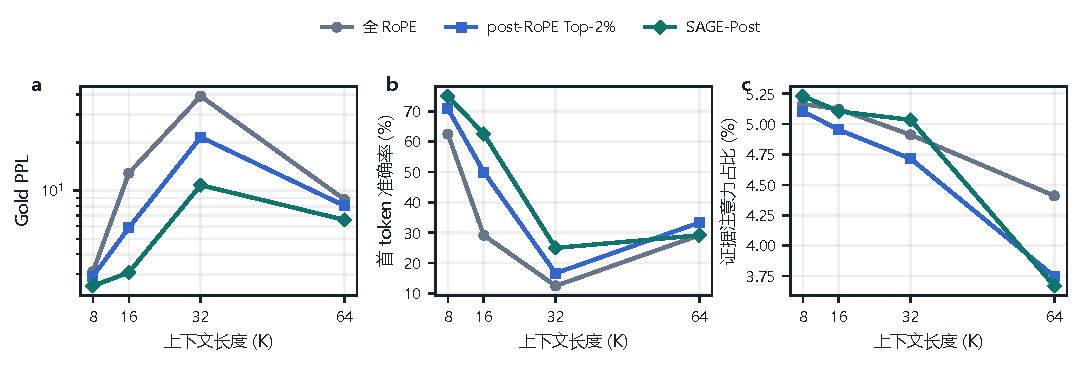
\includegraphics[width=\linewidth]{figures/heldout_results_zh.pdf}
  \caption{留出的两跳结果（每个长度使用 24 个种子）。对于 \GoldPPL，数值
  越低越好；对于其余指标，数值越高越好。SAGE-Post 在 16K 和 32K 时表现
  最强。相位敏感机制预期会产生非单调曲线，因此不能将该问题简单概括为随距离
  单调衰减。}
  \label{fig:heldout}
\end{figure}

\begin{table}[t]
  \caption{留出样例上的金标准答案质量。准确率为精确的首词元准确率。所有方法
  使用相同的提示；稀疏方法在每层、每个查询头中均保留 2\% 的词元。}
  \label{tab:quality}
  \centering
  \small
  \setlength{\tabcolsep}{4.1pt}
  \begin{tabular}{r rr rr rr}
    \toprule
    & \multicolumn{2}{c}{全注意力 RoPE}
    & \multicolumn{2}{c}{post-RoPE Top-2\%}
    & \multicolumn{2}{c}{\methodpost}\\
    \cmidrule(lr){2-3}\cmidrule(lr){4-5}\cmidrule(lr){6-7}
    长度 & PPL & 准确率 & PPL & 准确率 & PPL & 准确率\\
    \midrule
    8K  & 3.120  & 62.5 & 2.914  & 70.8 & \textbf{2.541}  & \textbf{75.0}\\
    16K & 12.885 & 29.2 & 5.858  & 50.0 & \textbf{3.080}  & \textbf{62.5}\\
    32K & 39.079 & 12.5 & 21.636 & 16.7 & \textbf{10.840} & \textbf{25.0}\\
    64K & 8.823  & 29.2 & 8.063  & \textbf{33.3} & \textbf{6.573} & 29.2\\
    \bottomrule
  \end{tabular}
\end{table}

在四个长度的点估计上，\methodpost 的 \GoldPPL 均优于全注意力，并在四个
长度中的三个上提高了首词元准确率（\cref{tab:quality}）。当每个长度--种子
数据点具有相同权重时，几何 \GoldPPL 从 10.851 降至 4.859，平均准确率从
33.3\% 提升至 47.9\%。与全注意力相比，8K、16K 和 32K 上的提升具有统计
显著性；在 64K 上，NLL 区间为 $[-0.615,0.004]$，尚不足以证明可靠增益。

更严格的比较对象是精确 post-RoPE Top-2\%，它在相同预算下单独考察候选
选择的影响。在 16K 上，\methodpost 将平均 NLL 降低 0.643（95\% 置信区间
$[-0.973,-0.342]$），相当于几何平均意义下 $1.90\times$ 的质量比。在 32K
上，NLL 降低 0.691（$[-1.035,-0.308]$），对应 $2.00\times$。8K 和 64K
的置信区间均跨越零。因此，当前证据支持的是存在一个长程补偿区间，而非
\methodpost 可以无条件取代 post-RoPE 选择。

\begin{table}[t]
  \caption{候选与注意力诊断指标。召回率表示金标准证据词元的召回比例；双链
  表示同时命中两行证据的层--头数据行比例；证据注意力表示 softmax 后落在
  金标准证据上的注意力占比。}
  \label{tab:mechanism-metrics}
  \centering
  \small
  \setlength{\tabcolsep}{4.4pt}
  \begin{tabular}{r l rrr}
    \toprule
    长度 & 方法 & 召回率 (\%) & 双链 (\%) & 证据注意力 (\%)\\
    \midrule
    \multirow{2}{*}{8K}
      & post-RoPE Top-2\% & 32.10 & 64.48 & 5.11\\
      & \methodpost        & 14.07 & 55.72 & 5.23\\
    \midrule
    \multirow{2}{*}{16K}
      & post-RoPE Top-2\% & 35.64 & 60.00 & 4.95\\
      & \methodpost        & \textbf{40.50} & \textbf{78.56} & \textbf{5.11}\\
    \midrule
    \multirow{2}{*}{32K}
      & post-RoPE Top-2\% & 38.98 & 60.59 & 4.72\\
      & \methodpost        & \textbf{46.71} & \textbf{80.05} & \textbf{5.04}\\
    \midrule
    \multirow{2}{*}{64K}
      & post-RoPE Top-2\% & 35.12 & 54.92 & \textbf{3.75}\\
      & \methodpost        & \textbf{44.45} & \textbf{78.16} & 3.67\\
    \bottomrule
  \end{tabular}
\end{table}

内部指标进一步定位了收益来源。在配对 NLL 得到可靠改善的 16K 和 32K 上，
\methodpost 同时提高了词元召回率、双链完成率和证据注意力
（\cref{tab:mechanism-metrics}）。在 64K 上，它提高了召回率与双链完成率，
却未提高证据注意力或准确率；这表明，当入选证据获得的 post-RoPE 权重仍然
较弱时，仅恢复候选并不足以改善输出。在 8K 上，较低的词元召回率与更优的 PPL
同时出现，说明不区分证据跨度内部差异的召回率，并不能完整代理与答案相关的
注意力头行为。这些例外具有启发性：它们支持采用距离感知且头感知的门控，而非
普遍启用的语义分支。

\subsection{消融实验与尚待完成的验证}

校准后的 pre/post 分数混合，以及保持注意力占比的远程重排序，在先导实验的
汇总点估计上优于 \methodpost；但它们会修改预训练注意力 logit，因此仅作为
附录消融。我们选择 \methodpost 作为主要结果，是因为它能够提供最清晰的
因果归因。

当前评测有意限定在较窄范围内。\todoexp{在相同的配对实验协议下加入 RULER
和一个自然多跳基准。}
\todoexp{在至少一种原生长上下文 RoPE 架构上复现实验。}
\todoexp{测量短上下文语言模型 PPL，并评测局部顺序任务。}
\todoexp{用近似索引替代精确的语义候选扫描，并测量端到端系统成本。}
在完成这些测试之前，我们的方法主张仅限于受控的长程证据检索场景。
